\documentclass[a4paper,11pt]{article}
\usepackage[T1]{fontenc}
\usepackage[polish]{babel}
\usepackage{lmodern}
\usepackage{amsmath}
\usepackage{graphicx}
\usepackage{booktabs}
\usepackage[margin=2.45cm]{geometry}
\usepackage{microtype}
\usepackage[hidelinks]{hyperref}

\title{Okres wahadła a jego długość\\\large Przykład odtwarzalnego miniartykułu}
\author{Opracowanie przykładowe do kursu „Programy użytkowe”}
\date{27 października 2026}

\begin{document}
\maketitle

\begin{abstract}
Porównuję pięć \emph{syntetycznych danych dydaktycznych} z modelem okresu
wahadła matematycznego dla małych wychyleń. Celem jest przećwiczenie
struktury artykułu, odwołań, bibliografii i odtwarzalnego wykresu.
Największa bezwzględna różnica między tabelą a przyjętym modelem jest
mniejsza niż $0{,}006\,\mathrm{s}$. Nie wyciągam z tego wniosku o jakości
rzeczywistego doświadczenia, ponieważ dane nie pochodzą z pomiaru.
\end{abstract}

\section{Pytanie i zakres}\label{sec:pytanie}
Pytanie brzmi: jak zmienia się okres $T$ wahadła, gdy zwiększamy jego
długość $L$? Materiał źródłowy OpenStax omawia wahadło matematyczne i
przybliżenie małych wychyleń~\cite{openstax_pendulum}. W tym ćwiczeniu
używam pięciu liczb przygotowanych na potrzeby kursu. Nie są to wyniki
laboratoryjne ani dane z cytowanego podręcznika.

Raport obejmuje:
\begin{itemize}
  \item zapis modelu z jednostkami,
  \item tabelę danych i rysunek z ich porównaniem,
  \item kontrolę różnic między danymi a modelem.
\end{itemize}

\section{Model}\label{sec:model}
Dla małego kąta wychylenia okres wahadła o długości $L$ przyjmuję jako
\begin{equation}
  T_{\mathrm{model}}(L)=2\pi\sqrt{\frac{L}{g}},
  \label{eq:okres}
\end{equation}
gdzie $g=9{,}81\,\mathrm{m/s^2}$. Zależność z
równania~\eqref{eq:okres} nie jest liniowa w $L$. Na przykład podwojenie
długości mnoży okres przez $\sqrt{2}$, a nie przez dwa. Wymiar pod
pierwiastkiem to $\mathrm{s^2}$, zatem wymiar $T$ to sekunda.

\section{Dane i metoda}\label{sec:metoda}
\subsection{Dane wejściowe}
Tabela~\ref{tab:dane} jest zapisana także w pliku \texttt{dane.csv}.
Kolumna $L$ podaje metry, a kolumna $T$ sekundy. Nie przypisuję tym
liczbom niepewności pomiarowej, bo nie znam sposobu ich uzyskania.

\begin{table}[htbp]
  \centering
  \begin{tabular}{cc}
    \toprule
    Długość $L$ (m) & Przykładowy okres $T$ (s) \\
    \midrule
    $0{,}20$ & $0{,}90$ \\
    $0{,}40$ & $1{,}27$ \\
    $0{,}60$ & $1{,}55$ \\
    $0{,}80$ & $1{,}80$ \\
    $1{,}00$ & $2{,}01$ \\
    \bottomrule
  \end{tabular}
  \caption{Syntetyczne dane użyte w przykładzie.}
  \label{tab:dane}
\end{table}

\subsection{Procedura odtworzenia rysunku}
\begin{enumerate}
  \item Wczytuję plik \texttt{dane.csv} do programu Python.
  \item Liczę krzywą z równania~\eqref{eq:okres} dla gęstej siatki $L$.
  \item Zapisuję punkty i krzywą w \texttt{wykres.pdf} oraz
        \texttt{wykres.png}.
\end{enumerate}
Skrypt \texttt{generuj\_wykres.py} korzysta z Matplotlib do budowy
wykresu; dokumentacja biblioteki opisuje użyte polecenie rysujące
linię~\cite{matplotlib_plot}. Plik PDF zawiera osie i legendę w postaci
łatwej do powiększenia.

\section{Wyniki}\label{sec:wyniki}
Na rysunku~\ref{fig:okres} punkty rosną wraz z długością, podobnie jak
krzywa modelowa. Rozdzielam te dwa źródła informacji różnymi znakami:
punkty oznaczają tabelę, a linia przedstawia wzór.

\begin{figure}[htbp]
  \centering
  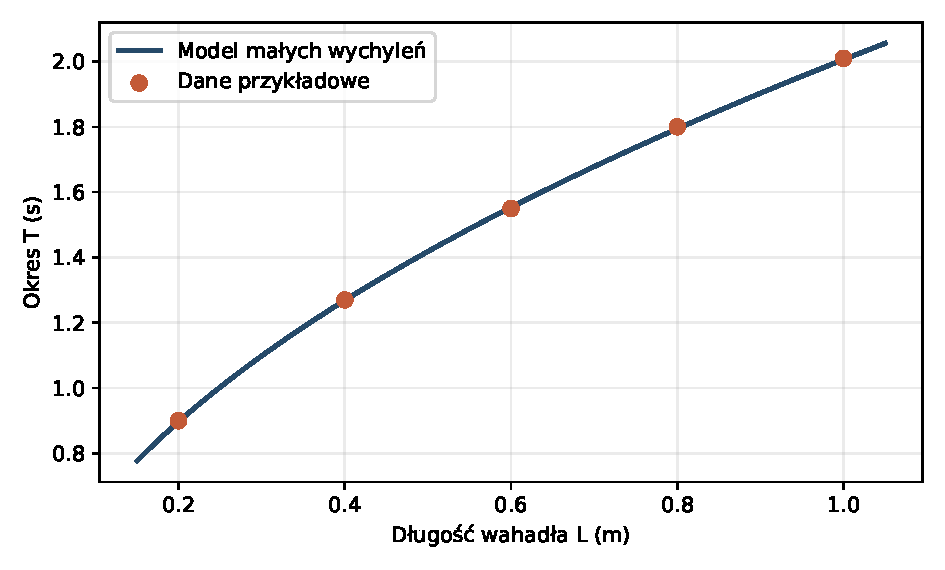
\includegraphics[width=0.88\linewidth]{wykres.pdf}
  \caption{Przykładowe okresy i model małych wychyleń; osie podają
  wielkości oraz jednostki.}
  \label{fig:okres}
\end{figure}

Różnicę dla $i$-tego wiersza definiuję jako
\[
  r_i=T_i-T_{\mathrm{model}}(L_i).
\]
Największe $|r_i|$ wynosi około $0{,}00572\,\mathrm{s}$. Dla
$L=1{,}00\,\mathrm{m}$ model daje około $2{,}0061\,\mathrm{s}$, a
tabela podaje $2{,}01\,\mathrm{s}$. Porównanie jest więc spójne na
poziomie zaokrąglenia danych w tabeli.

\section{Ograniczenia i wniosek}\label{sec:wniosek}
Model wymaga małych wychyleń, pomijalnej masy nici i zaniedbania oporu.
Tutaj dodatkowym ograniczeniem jest brak protokołu pomiarowego. Nie znam
liczby powtórzeń, sposobu wyznaczania okresu ani niepewności. Nie mogę
więc ocenić zgodności eksperymentu z teorią ani przypisywać małych
różnic konkretnemu zjawisku fizycznemu.

W ramach ćwiczenia z tabeli~\ref{tab:dane} i rysunku~\ref{fig:okres}
wynika jedynie, że przygotowane liczby rosną zgodnie z trendem modelu
z równania~\eqref{eq:okres}. \emph{Źródło danych i ograniczenia muszą
pozostać widoczne także wtedy, gdy wykres wygląda przekonująco.}

\bibliographystyle{plain}
\bibliography{references}
\end{document}
